\documentclass[aspectratio=169, table, 12pt]{beamer}

\usepackage{colortbl}
\usepackage{xcolor}
\usepackage{listings}
\usepackage{tabularx}
\usepackage{tikz}
\usetikzlibrary{arrows.meta, positioning, calc, fit,
  shapes.geometric, backgrounds}

\makeatletter
\def\input@path{{../theme/}}
\makeatother
\graphicspath{{../theme/}{../../figures/}}
\usetheme{Pradita}

\definecolor{praditagreen}{RGB}{37, 113, 71}

% Tema membuat garis tabel berwarna putih. Dikembalikan agar tabel terbaca.
\arrayrulecolor{black}
\setlength{\arrayrulewidth}{0.5pt}

\lstdefinestyle{PythonStyle}{
  language=Python,
  basicstyle=\ttfamily\scriptsize,
  keywordstyle=\color{blue}\bfseries,
  commentstyle=\color{gray}\itshape,
  stringstyle=\color{red},
  breaklines=true,
  frame=lines,
  backgroundcolor=\color{lightgray!10},
  tabsize=2,
  showstringspaces=false
}

\lstdefinelanguage{bash}{
  keywords={},
  basicstyle=\ttfamily\scriptsize,
  ndkeywords={cd, python, bash, source},
  ndkeywordstyle=\color{purple}\bfseries,
  sensitive=true,
  commentstyle=\color{gray},
  breaklines=true,
  frame=lines,
  backgroundcolor=\color{lightgray!10},
  tabsize=2,
  comment=[l]{\#},
  showstringspaces=false
}

\title{\Huge{Pengenalan dan Client-Server}}
\subtitle{IF231303 Arsitektur Perangkat Lunak}
\author{Alfa Yohannis}

\begin{document}

\frame{\titlepage}

\begin{frame}{{\Large Tujuan Pembelajaran}}
  \vspace{10pt}
  \begin{enumerate}
    \item Menjelaskan arti arsitektur perangkat lunak beserta aspek yang
          membedakannya dari rancangan rinci.
    \item Membedakan tanggung jawab klien dari tanggung jawab server pada
          arsitektur client-server.
    \item Mengukur waktu bolak-balik satu \textit{request} dan perubahannya
          ketika jumlah klien bertambah.
  \end{enumerate}

  \vspace{10pt}
  {\small Contohnya satu server konversi kurs yang dipanggil banyak klien.}
\end{frame}

\begin{frame}{{\Large Pendahuluan}}
  \vspace{8pt}
  \begin{itemize}\small
    \item Setiap sistem punya arsitektur, baik dirancang maupun tidak, yaitu
          susunan bagian besarnya beserta aturan hubungan di antaranya.
    \item Yang membedakannya dari rancangan rinci adalah biaya perubahan.
          Mengganti nama fungsi murah, sedangkan memecah sistem menjadi
          beberapa layanan menyentuh hampir seluruh \textit{file}.
    \item Keputusan yang mahal diubah itulah keputusan arsitektural.
    \item Bab ini mengikuti kerangka Richards dan Ford, lalu membahas bentuk
          pertama yang menjadi dasar bab berikutnya, yaitu client-server.
  \end{itemize}
\end{frame}

\begin{frame}{{\Large Aspek yang Dinilai}}
  \vspace{4pt}
  \centering
  \footnotesize
  \begin{tabularx}{\textwidth}{|l|X|X|}
    \hline
    \textbf{Aspek} & \textbf{Pertanyaannya} & \textbf{Diukur dengan} \\
    \hline
    Kemudahan perawatan & Berapa banyak \textit{file} berubah untuk satu
      \textit{change request}? & Jumlah \textit{file} dan baris \\
    \hline
    Kemampuan skala & Apa yang terjadi ketika jumlah pengguna naik sepuluh
      kali? & Latensi pada beban bertingkat \\
    \hline
    Kinerja & Berapa lama satu \textit{request} dilayani? & Median dan
      persentil ke-95 \\
    \hline
    Ketersediaan & Apa yang gagal ketika satu bagian mati? & Jumlah proses
      yang terhenti \\
    \hline
    Kemudahan pengujian & Berapa besar bagian yang dapat diuji tanpa
      infrastruktur? & Cakupan pengujian \\
    \hline
  \end{tabularx}
\end{frame}

\begin{frame}{{\Large Aspek yang Saling Bertentangan}}
  \vspace{8pt}
  \begin{itemize}\small
    \item Arsitektur tidak dinilai benar atau salah, melainkan sesuai atau
          tidak dengan kebutuhannya.
    \item Menaikkan kemampuan skala biasanya menurunkan kemudahan perawatan,
          sebab sistem dipecah menjadi lebih banyak bagian.
    \item Menaikkan kinerja sering menurunkan kemudahan pengujian, sebab jalan
          pintas mulai bermunculan.
    \item Pekerjaan arsitek karena itu adalah memilih aspek mana yang
          dikorbankan.
  \end{itemize}

  \vspace{8pt}
  {\small Setiap bab pada modul ini mengukur dua atau tiga aspek tersebut, agar
  perbandingannya berdiri di atas angka.}
\end{frame}

\begin{frame}{{\Large Arsitektur Client-Server}}
  \vspace{4pt}
  \centering
  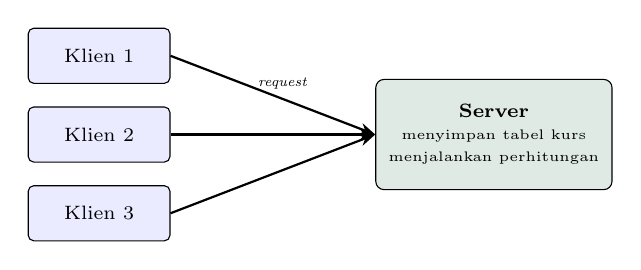
\begin{tikzpicture}[
    kotak/.style={draw, rounded corners=2pt, minimum width=1.8cm,
      minimum height=0.7cm, align=center, font=\scriptsize},
    server/.style={draw, rounded corners=3pt, minimum width=3.0cm,
      minimum height=1.4cm, align=center, font=\scriptsize, fill=praditagreen!15},
    panah/.style={-{Stealth[length=2mm]}, thick}
  ]
    \node[server] (srv) {\textbf{Server}\\
      {\tiny\mdseries menyimpan tabel kurs}\\
      {\tiny\mdseries menjalankan perhitungan}};

    \node[kotak, fill=blue!8, left=2.6cm of srv, yshift=1.0cm] (k1) {Klien 1};
    \node[kotak, fill=blue!8, left=2.6cm of srv] (k2) {Klien 2};
    \node[kotak, fill=blue!8, left=2.6cm of srv, yshift=-1.0cm] (k3) {Klien 3};

    \draw[panah] (k1.east) -- node[above, font=\tiny, pos=0.55] {\textit{request}} (srv.west);
    \draw[panah] (k2.east) -- (srv.west);
    \draw[panah] (k3.east) -- (srv.west);
  \end{tikzpicture}

  \vspace{6pt}
  \raggedright
  {\small Klien meminta, server melayani. Seluruh \textit{request} berawal dari
  klien, dan server tidak pernah memanggil klien. Fielding menelusuri
  pembatasan pemisahan ini, termasuk biaya jaringan yang tidak dapat dihapus.}
\end{frame}

\begin{frame}{{\Large Siapa Menyimpan Apa}}
  \vspace{8pt}
  \begin{itemize}\small
    \item Server menyimpan data bersama dan menjalankan aturan bisnis.
    \item Klien menyimpan keadaan tampilan saja. Klien pada contoh bab ini
          hanya menyusun alamat, mengirim \textit{request}, lalu menampilkan
          jawabannya.
    \item Tabel kurs hanya ada di server, sehingga memperbaruinya cukup di satu
          tempat dan seluruh klien langsung memakai nilai barunya.
  \end{itemize}
\end{frame}

\begin{frame}[fragile]{{\Large Kode: Penangan \textit{Request}}}
  \vspace{2pt}
\begin{lstlisting}[style=PythonStyle]
def do_GET(self):
  """Membaca parameter request, menghitung, lalu membalas dalam JSON."""
  alamat = urlparse(self.path)
  parameter = parse_qs(alamat.query)
  asal = parameter.get("asal", ["USD"])[0]
  tujuan = parameter.get("tujuan", ["IDR"])[0]
  teks_nominal = parameter.get("nominal", ["1"])[0]
  nominal = float(teks_nominal)

  hasil = hitung_konversi(asal, tujuan, nominal)
  if hasil is None:
    self.kirim(404, {"galat": "Kurs tidak tersedia"})
  else:
    self.kirim(200, {"asal": asal, "tujuan": tujuan, "hasil": hasil})
\end{lstlisting}

  {\small Potongan dari \texttt{server.py}. Balasannya berbentuk JavaScript
  Object Notation (JSON).}
\end{frame}

\begin{frame}{{\Large Dua Biaya yang Melekat}}
  \vspace{8pt}
  \begin{itemize}\small
    \item \textbf{Biaya perjalanan.} Setiap \textit{request} menempuh jaringan
          pergi dan pulang. Pada server di kota lain, biaya ini menjadi bagian
          terbesar waktu tanggap dan tidak hilang walaupun perhitungannya
          dipercepat.
    \item \textbf{Biaya antrean.} Satu server melayani banyak klien. Ketika
          \textit{request} datang lebih cepat daripada kemampuan server, sisanya
          menunggu.
    \item Server contoh melayani satu \textit{request} pada satu waktu,
          sehingga gejala antrean muncul jelas begitu klien bertambah.
  \end{itemize}
\end{frame}

\begin{frame}{{\Large Analogi: Warung dengan Satu Kasir}}
  \vspace{8pt}
  \begin{itemize}\small
    \item Pembeli antre dan memesan, kasir yang menghitung dan menyimpan uang.
    \item Pembeli tidak perlu tahu harga pokok setiap barang, dan perubahan
          harga cukup diberitahukan kepada kasir.
    \item Kelemahannya sama, yaitu ketika pembeli banyak, antrean memanjang
          walaupun setiap pesanan sebenarnya cepat dilayani.
  \end{itemize}
\end{frame}

\begin{frame}{{\Large Kasus: Tiga Kejadian}}
  \vspace{6pt}
  \begin{itemize}\small
    \item \textbf{Netflix, 2008.} Kerusakan basis data menghentikan pengiriman
          Digital Versatile Disc (DVD) selama tiga hari. Aplikasinya yang
          semula satu kesatuan lalu dipecah menjadi ratusan layanan kecil.
    \item \textbf{HealthCare.gov, 2013.} Setiap pengunjung wajib membuat akun
          lewat satu sistem pintu masuk. 250.000 pengguna datang serentak, dan
          hanya enam orang selesai mendaftar pada hari pertama.
    \item \textbf{Transfer antarbank.} Sistem Kliring Nasional Bank Indonesia
          (SKNBI) beroperasi pukul 06.30 sampai 16.30 mengikuti jendela waktu.
          Sejak 21 Desember 2021, BI-FAST menyelesaikan setiap transfer
          seketika, setiap saat.
  \end{itemize}

  \vspace{6pt}
  {\small Yang menentukan bukan algoritmanya, melainkan susunan komponen dan
  cara komponen itu saling menunggu.}
\end{frame}

\begin{frame}{{\Large Hasil: Latensi dan Jumlah Klien}}
  \vspace{6pt}
  \centering
  \small
  \begin{tabularx}{0.8\textwidth}{|X|l|l|}
    \hline
    \textbf{Jumlah klien serentak} & \textbf{Median (ms)} & \textbf{Terbesar (ms)} \\
    \hline
    1 & 0,310 & 10,023 \\
    \hline
    2 & 0,428 & 0,623 \\
    \hline
    4 & 0,681 & 1,405 \\
    \hline
    8 & 1,181 & 1064,106 \\
    \hline
    16 & 1,358 & 1050,540 \\
    \hline
  \end{tabularx}

  \vspace{6pt}
  {\small Setiap klien mengirim dua puluh \textit{request} berurutan ke server
  yang sama.}
\end{frame}

\begin{frame}{{\Large Membaca Hasilnya}}
  \vspace{10pt}
  \begin{itemize}\small
    \item Median hanya naik dari 0,31 menjadi 1,36 ms, sedangkan nilai
          terbesarnya melonjak mulai delapan klien sampai melampaui seribu
          milidetik.
    \item Sebabnya antrean sambungan \texttt{HTTPServer} yang hanya muat lima.
          Dengan antrean 64, nilai terbesar pada 16 klien turun menjadi 5,795
          ms, sedangkan mediannya naik menjadi 2,999 ms.
    \item Sebagian kecil \textit{request} menunggu sangat lama, sedangkan
          sebagian besar lainnya tetap cepat.
  \end{itemize}

  \vspace{10pt}
  {\small Gejala itu hilang bila yang dilaporkan hanya rata-rata. Karena itu
  setiap pengukuran pada modul ini menyertakan nilai terbesar atau persentil
  ke-95.}
\end{frame}

\begin{frame}{{\Large Kelebihan dan Kekurangan}}
  \vspace{4pt}
  \centering
  \footnotesize
  \begin{tabularx}{\textwidth}{|X|X|}
    \hline
    \textbf{Kelebihan} & \textbf{Kekurangan} \\
    \hline
    Data bersama disimpan di satu tempat, sehingga pembaruan cukup sekali &
      Server menjadi satu-satunya titik yang bila mati menghentikan seluruh
      layanan \\
    \hline
    Aturan bisnis tidak dapat diubah dari sisi klien & Setiap \textit{request}
      menanggung biaya perjalanan jaringan \\
    \hline
    Klien menjadi ringan dan mudah diganti & Server menjadi antrean bersama
      ketika klien bertambah \\
    \hline
    Perangkat klien tidak perlu bertenaga besar & Menambah kemampuan server
      lebih mahal daripada menambah klien \\
    \hline
  \end{tabularx}
\end{frame}

\begin{frame}{{\Large \textit{Summary}}}
  \vspace{10pt}
  \begin{itemize}\small
    \item Arsitektur adalah susunan bagian besar sistem, dan yang membedakannya
          dari rancangan rinci adalah biaya perubahannya.
    \item Aspek penilaiannya saling bertentangan, sehingga arsitek memilih
          aspek mana yang dikorbankan.
    \item Client-server menaruh data bersama dan aturan bisnis di server,
          sedangkan klien menyimpan keadaan tampilan saja.
    \item Pembagian itu menimbulkan biaya perjalanan dan biaya antrean.
  \end{itemize}

  \vspace{10pt}
  {\small Biaya antrean tidak terlihat pada median, tetapi tampak jelas pada
  nilai terbesar.}
\end{frame}

\begin{frame}[fragile]{{\Large Persiapan Latihan}}
  \vspace{5pt}
\begin{lstlisting}[language=bash]
bash sources/siapkan_venv.sh
source .venv/bin/activate
cd sources/chapter01
python server.py
# Server berjalan di http://127.0.0.1:8000
\end{lstlisting}

  \vspace{6pt}
  {\small Server dijalankan pada terminal pertama, skrip lainnya pada terminal
  kedua. Langkah lengkap, tabel contoh, dan lembar isian ada di modul Bab 1,
  yang menjadi rujukan utama latihan ini.}
\end{frame}

\begin{frame}[fragile]{{\Large Latihan 1: Tanggung Jawab}}
  \vspace{3pt}
\begin{lstlisting}[language=bash]
python klien.py USD IDR 100
# 100 USD = 1,625,000.00 IDR
# sesudah kurs USD diubah: 100 USD = 1,630,000.00 IDR
\end{lstlisting}

  \vspace{3pt}
  \begin{enumerate}\small
    \item Cari tabel kurs di dalam \texttt{klien.py}.
    \item Ubah satu nilai kurs di \texttt{server.py}, jalankan ulang server,
          lalu jalankan klien tanpa mengubah apa pun.
    \item Matikan server, lalu jalankan klien sekali lagi.
  \end{enumerate}

  \vspace{3pt}
  {\small Pertanyaan: apa untung dan rugi menyimpan tabel kurs hanya di
  server?}
\end{frame}

\begin{frame}[fragile]{{\Large Latihan 2: Biaya Perjalanan}}
  \vspace{3pt}
\begin{lstlisting}[language=bash]
python ukur_latensi.py
# Median           : 0.273 ms
# Persentil ke-95  : 0.335 ms
# Terbesar         : 9.353 ms
\end{lstlisting}

  \vspace{3pt}
  \begin{enumerate}\small
    \item Catat kelima angkanya, lalu ulangi pengukurannya tiga kali.
    \item Bandingkan nilai terkecil dengan nilai terbesar setiap pengukuran.
    \item Tambahkan perhitungan berulang di \texttt{hitung\_konversi}, lalu ukur
          kembali.
  \end{enumerate}

  \vspace{3pt}
  {\small Pertanyaan: bagian mana dari waktu itu yang tetap ada walaupun
  server dipercepat?}
\end{frame}

\begin{frame}[fragile]{{\Large Latihan 3: Menambah Klien}}
  \vspace{3pt}
\begin{lstlisting}[language=bash]
python ukur_beban.py
#  Klien   Median (ms)   Terbesar (ms)
#      4         0.681           1.405
#      8         1.181        1064.106
\end{lstlisting}

  \vspace{3pt}
  \begin{enumerate}\small
    \item Catat median dan nilai terbesar pada setiap jumlah klien.
    \item Tandai jumlah klien saat nilai terbesar mulai melonjak.
    \item Bandingkan pertumbuhan median dengan pertumbuhan nilai terbesar.
  \end{enumerate}

  \vspace{3pt}
  {\small Pertanyaan: aspek mana yang paling tertekan pada client-server,
  dan angka mana yang menjadi dasarnya?}
\end{frame}

\end{document}
